\documentclass[oneside,a4paper,14pt]{extarticle}
%\usepackage[T1,T2A,TU]{fontenc}
\usepackage[a4paper,letterpaper,top=20mm,bottom=20mm,left=20mm,right=10mm]{geometry}
\usepackage[russian]{babel}
%\usepackage{textcomp}
\usepackage{indentfirst}
\usepackage{graphicx}
%\usepackage{mwe}
%\usepackage{wrapfig}
\usepackage{caption}
%\usepackage{amsmath}
%\usepackage{amsfonts}
%\usepackage{amsthm}
%\usepackage{amssymb}
%\usepackage[all]{xy}
%\usepackage[breaklinks]{hyperref}
\usepackage{titlesec}
\usepackage{verbatim, fancyvrb}

\titleformat{\section} % Настройка формата заголовков секций
{\normalsize\bfseries} % Устанавливает размер шрифта на нормальный и делает его жирным
{\thesection} % Указывает, что номер секции будет отображаться перед заголовком
{1em} % Устанавливает расстояние между номером секции и заголовком в 1em
{} % Дополнительные параметры.

\titleformat{\subsection} % Настройка формата заголовков подсекций
{\normalsize\bfseries} % Устанавливает размер шрифта на нормальный и делает его жирным
{\thesubsection} % Указывает, что номер подсекции будет отображаться перед заголовком
{1em} % Устанавливает расстояние между номером подсекции и заголовком в 1em
{} % Дополнительные параметры.

\titleformat{\subsubsection} % Настройка формата заголовков подподсекций
{\normalsize\bfseries} % Устанавливает размер шрифта на нормальный и делает его жирным
{\thesubsection} % Указывает, что номер подподсекции будет отображаться перед заголовком
{1em} % Устанавливает расстояние между номером подподсекции и заголовком в 1em
{} % Дополнительные параметры.

\renewcommand\baselinestretch{1.45}\normalsize %межстр интервал
\setlength{\parindent}{1.25cm} %длина отступа нового абзаца

\begin{document}
\newpage
\thispagestyle{empty}
\begin{center}
	МИНИСТЕРСТВО НАУКИ И ВЫСШЕГО ОБРАЗОВАНИЯ\\
	РОССИЙСКОЙ ФЕДЕРАЦИИ
	ФЕДЕРАЛЬНОЕ ГОСУДАРСТВЕННОЕ БЮДЖЕТНОЕ\\
	ОБРАЗОВАТЕЛЬНОЕ
	УЧРЕЖДЕНИЕ ВЫСШЕГО ОБРАЗОВАНИЯ\\
	«ВЯТСКИЙ ГОСУДАРСТВЕННЫЙ УНИВЕРСИТЕТ»\\
	Институт математики и информационных систем\\
	Факультет автоматики и вычислительной техники\\
	Кафедра электронных вычислительных машин
\end{center}
\vspace{20mm}

\begin{center}
	Отчёт по лабораторной работе №3\\
	по дисциплине\\
	<<Программирование>>\\
\end{center}
\vspace{40mm}
\noindent
\begin{tabular}{ll}
	Разработал студент гр. ИВТб-1301-05-00 & \rule[-1mm]{30mm}{0.10mm}\,/Черкасов А. А./   \\
	                                       & \hspace{8mm}\footnotesize(подпись)            \\

	Заместитель кафедры ЭВМ                & \rule[-1mm]{30mm}{0.10mm}\,/Долженкова М. Л./ \\
	                                       & \hspace{8mm}\footnotesize(подпись)            \\
\end{tabular}

\vfill
\begin{center}
	Киров\\
	2024
\end{center}

\newpage\thispagestyle{plain}

\section*{Цель}

\sloppy Цель работы: Освоить синтаксис построения процедур и функций, изучить способы передачи данных в подпрограммы, получить навыки организации минимального пользовательского интерфейса.

\section*{Задание}
\begin{itemize}
    \item[$-$] Реализовать программу вычисления площади фигуры, ограниченной кривой $2 \times x^3 + 2 \times x^2 + 3 \times x + 1$ и осью OX (в положительной части оси OY).
    \item[$-$] Вычисление определенного интеграла должно выполняться численно, с приминением метода средних прямоугольников.
    \item[$-$] Пределы интегрирования вводятся пользователем.
    \item[$-$] Взаимодействие с пользователем должно осуществляться посредством case-меню.
    \item[$-$] Требуется реализовать возможность оценки погрешности полученного результата.
    \item[$-$] Необходимо использовать процедуры и функции там, где это целесообразно.

\end{itemize}

\section*{Решение}
\noindent Схема алгоритма Задания представлена на Рисунках 1.1, 1.2, 1.3.\\
\noindent Исходный код представлен в Приложении А1.\\
\newpage
\begin{figure}[!ht]
	\centering
	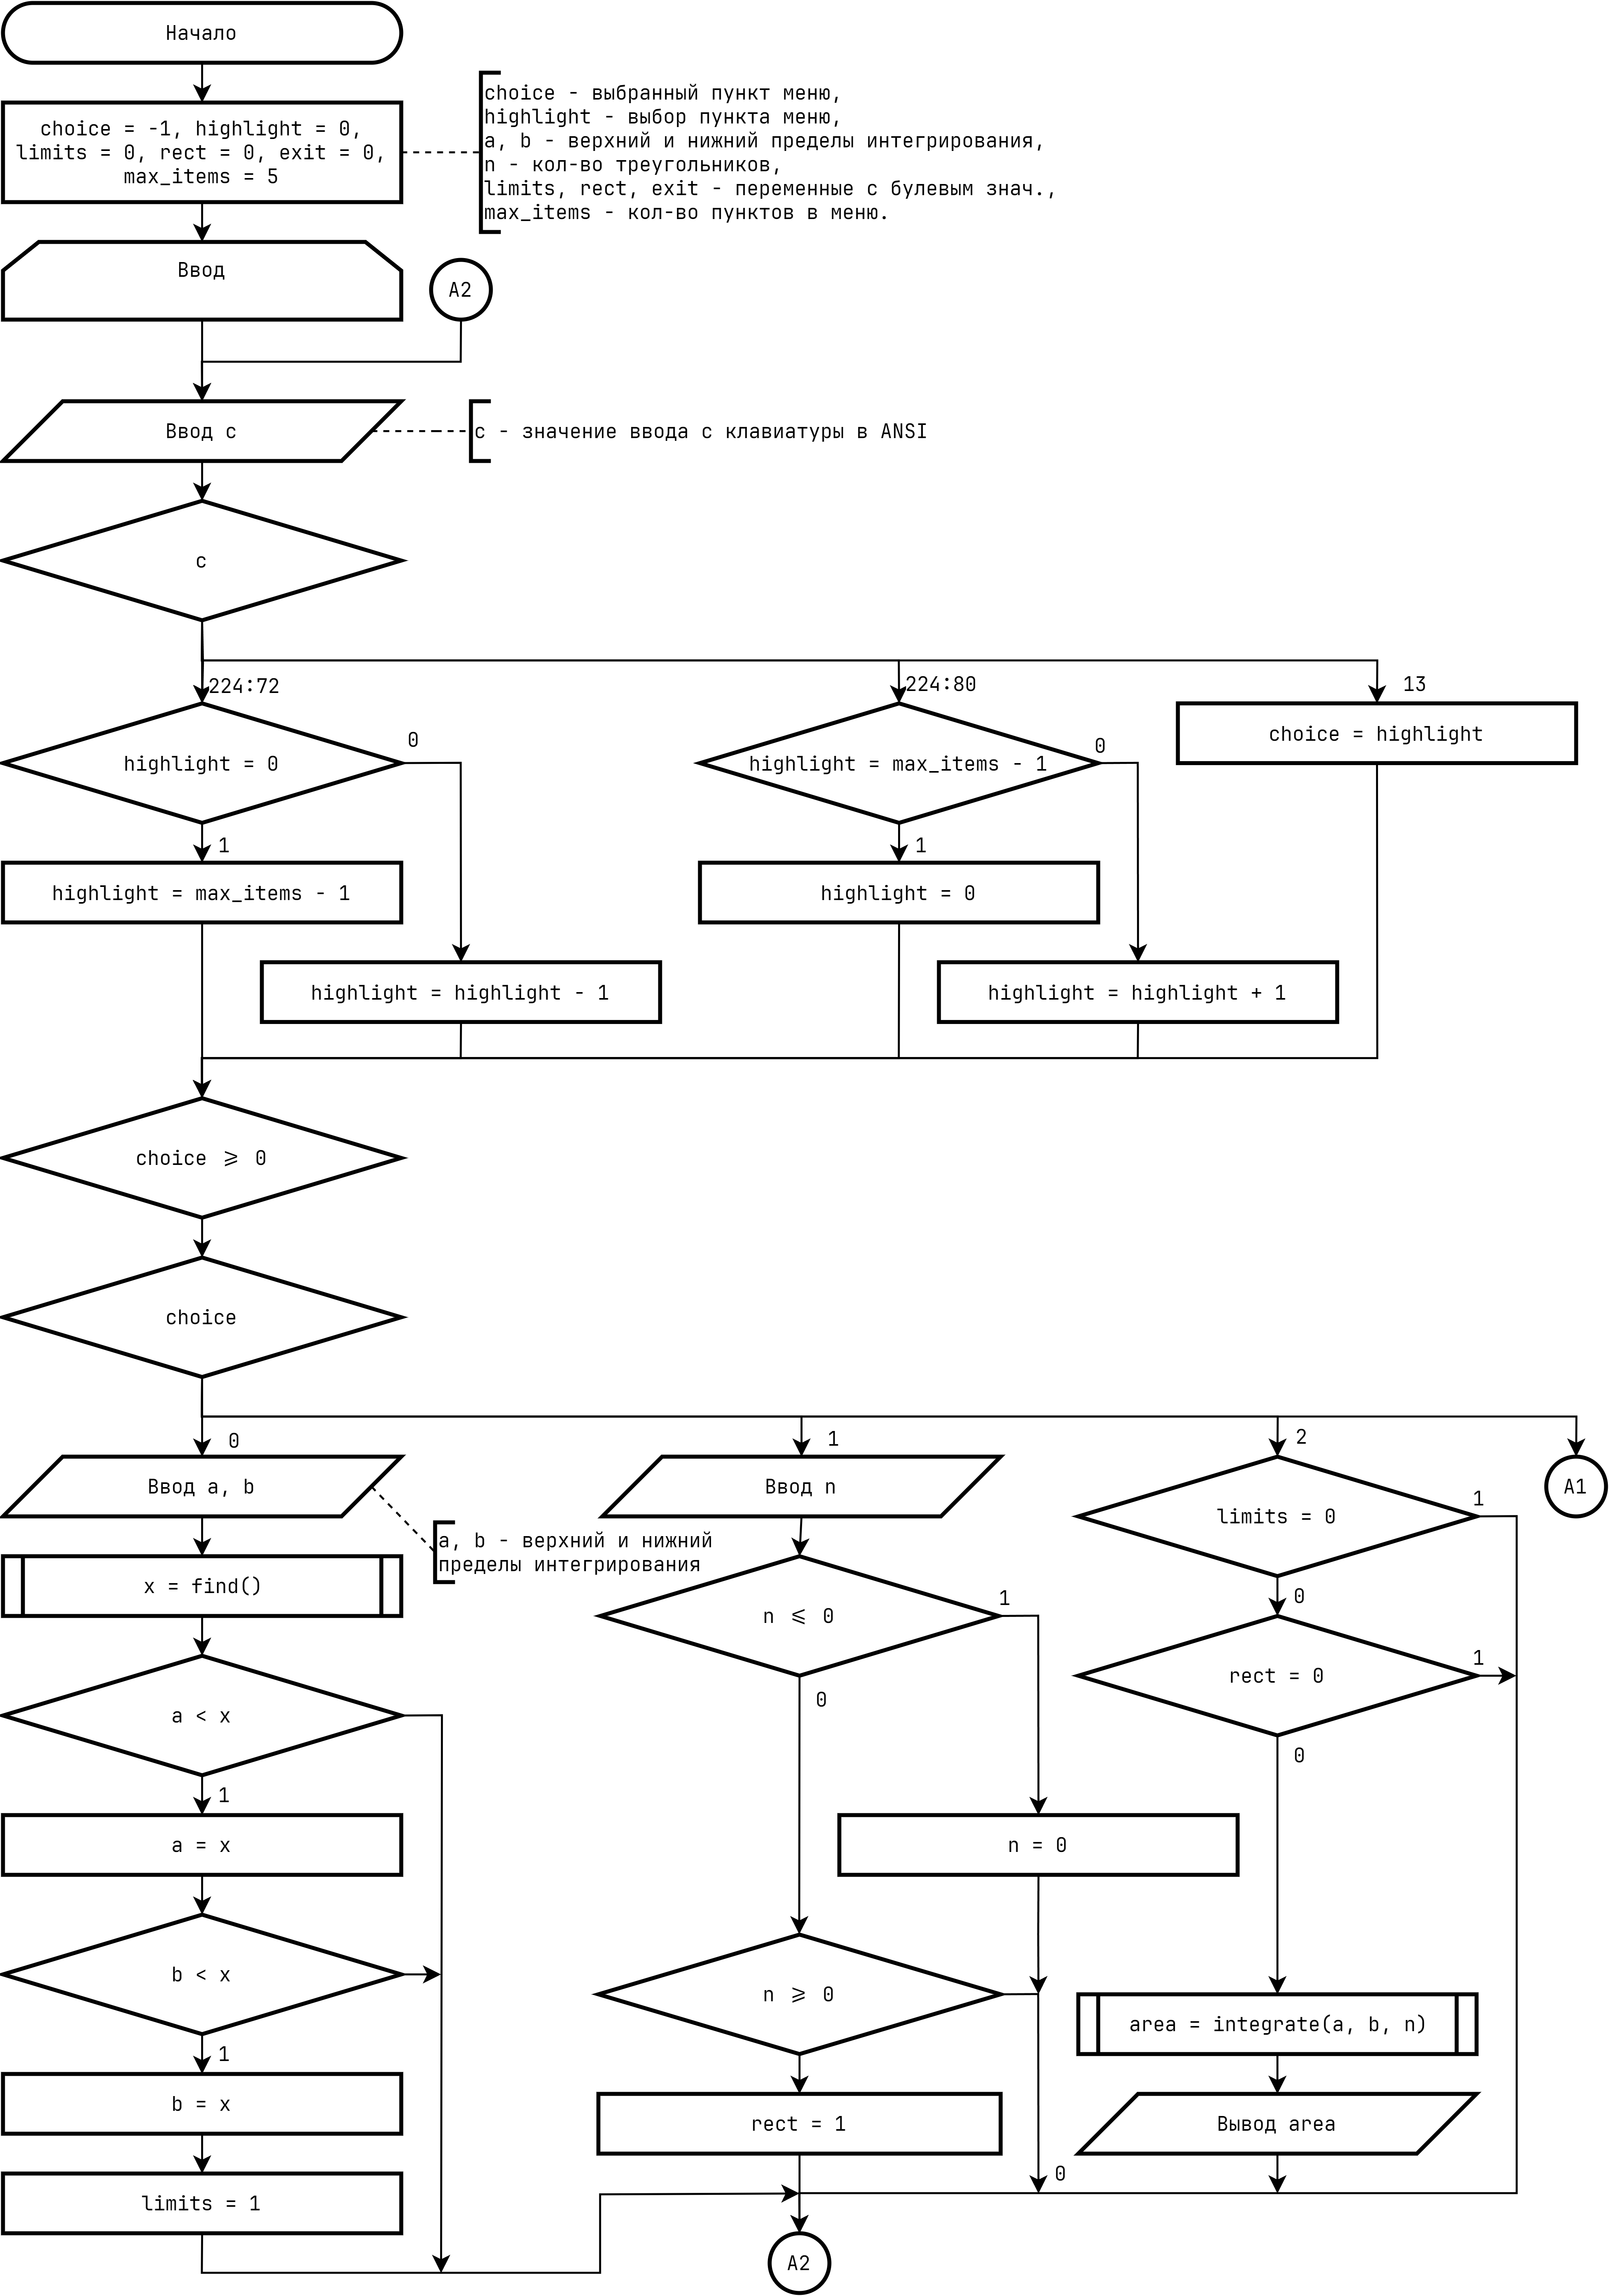
\includegraphics[width=0.8\textwidth]{pics/flowchart_p1.png}
	\caption*{Рисунок 1.1 - Схема алгоритма Задания.}
\end{figure}

\begin{figure}[!ht]
	\centering
	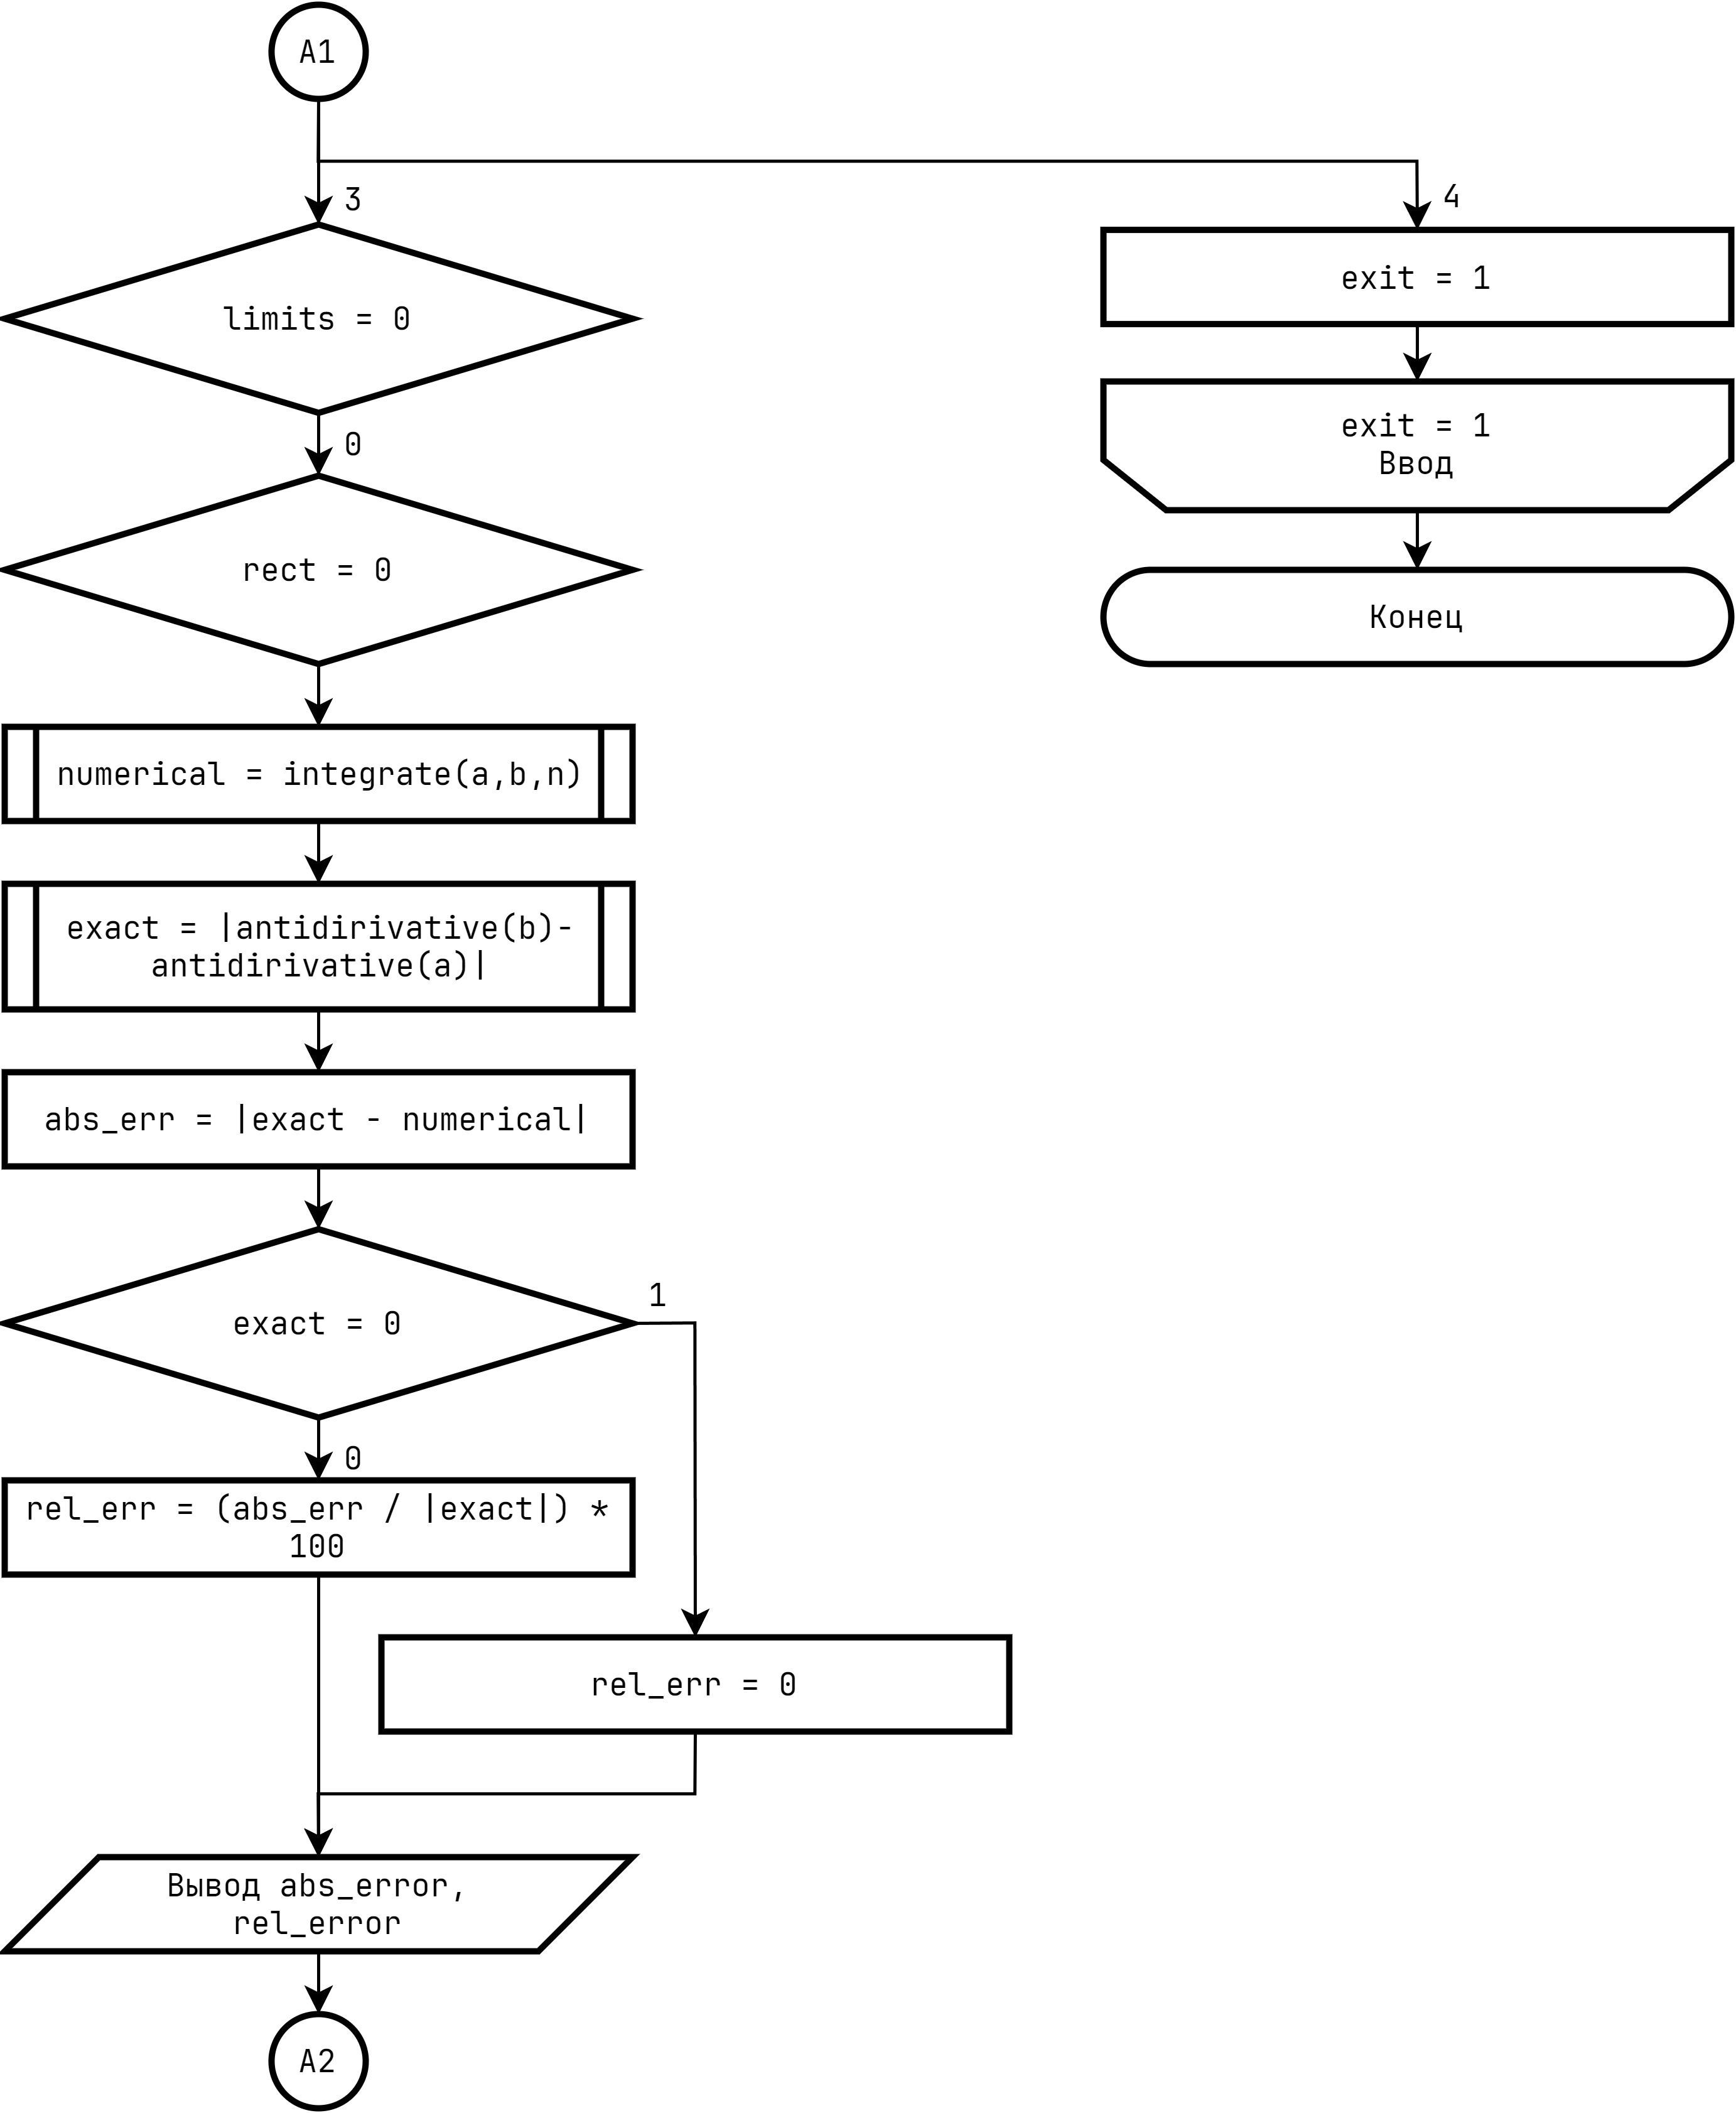
\includegraphics[height=0.9\textheight]{pics/flowchart_p2.png}
	\caption*{Рисунок 1.2 - Схема алгоритма Задания.}
\end{figure}

\begin{figure}[!ht]
	\centering
	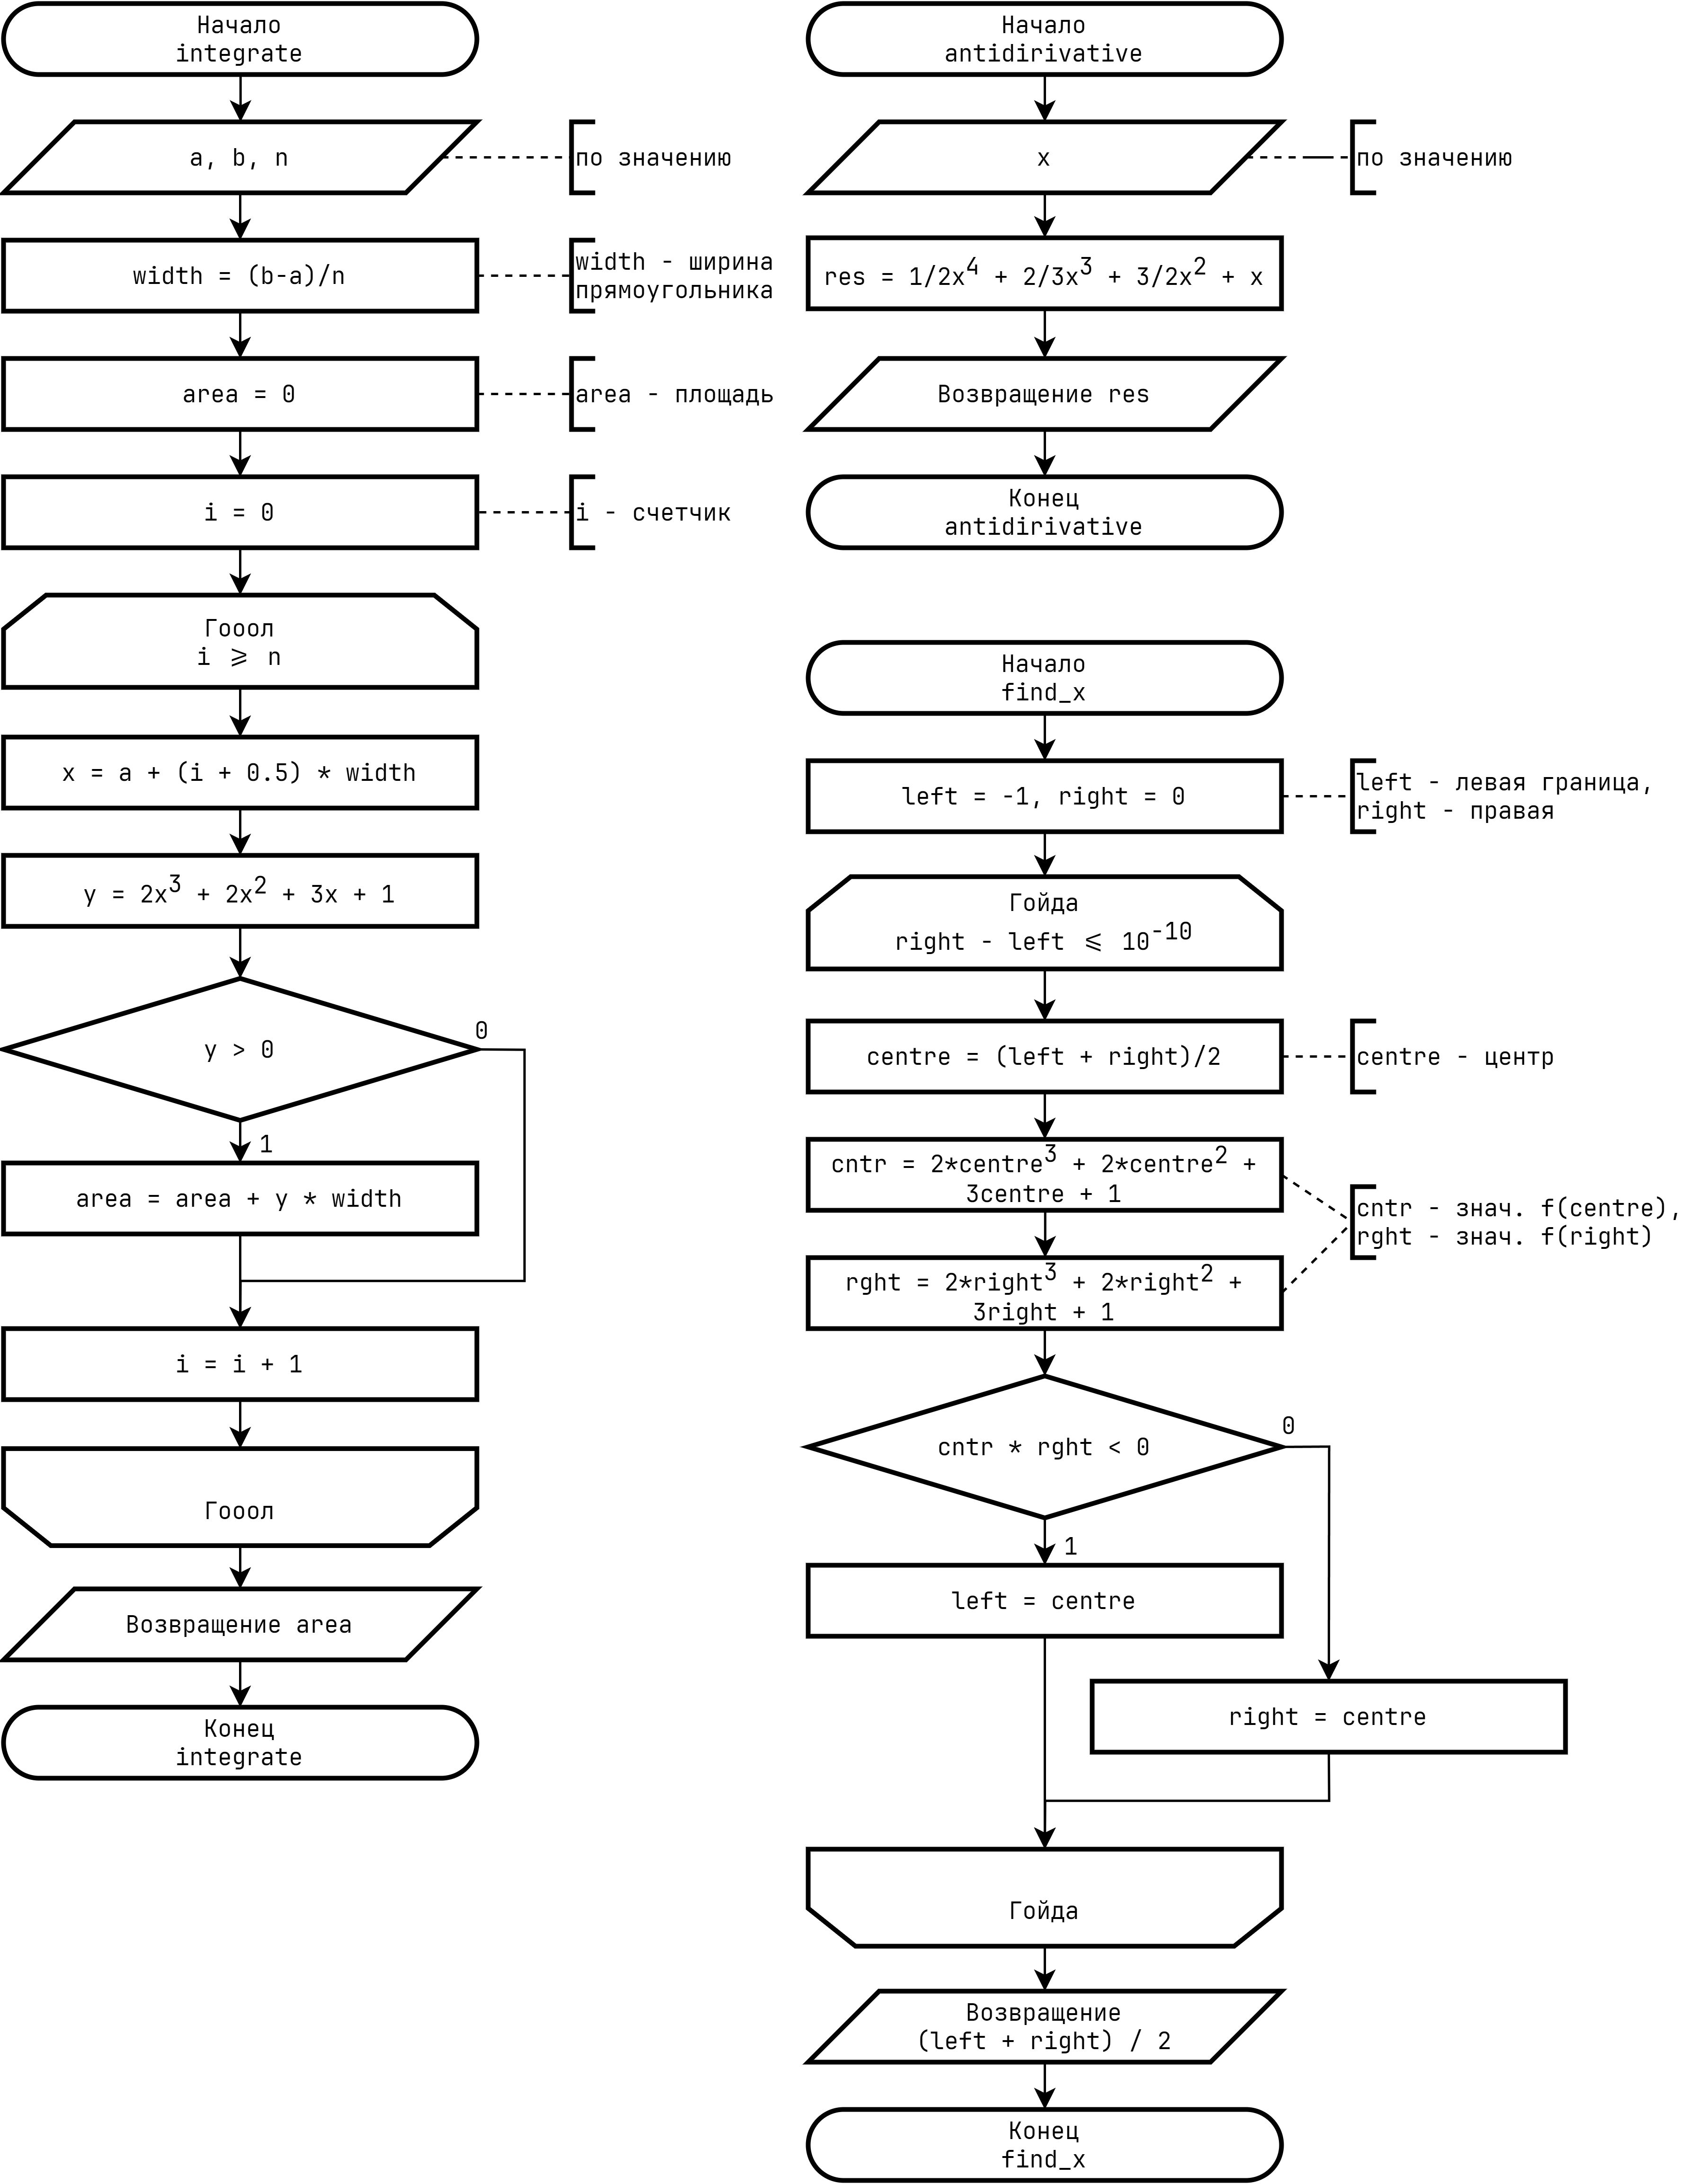
\includegraphics[height=0.9\textheight]{pics/flowchart_p3.png}
	\caption*{Рисунок 1.3 - Схема алгоритма Задания.}
\end{figure}

\section*{Вывод}
В ходе выполнения работы были освоены основы работы с функциями и процедурами, реализовано численное интегрирование методом средних прямоугольников, изучены подходы к организации пользовательского интерфейса.\\

\section*{Приложеие А1. Исходный код Задания.}
\VerbatimInput[fontsize=\small]{code/main.c}
\end{document}